\tikzset{every picture/.style={line width=0.75pt}} %set default line width to 0.75pt        

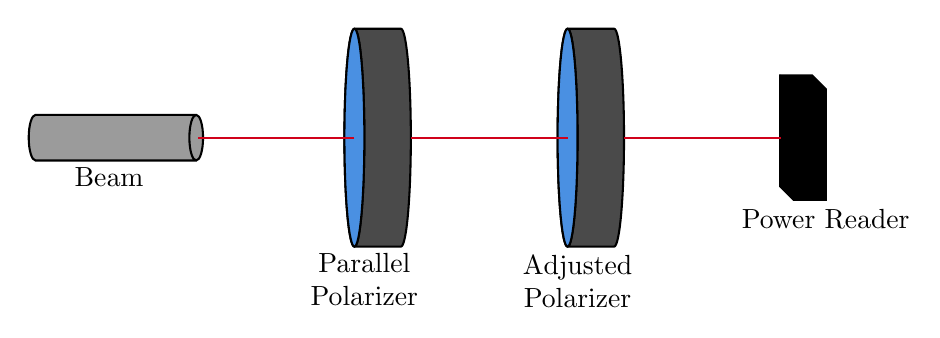
\begin{tikzpicture}[x=0.75pt,y=0.75pt,yscale=-1,xscale=1]
%uncomment if require: \path (0,504); %set diagram left start at 0, and has height of 504

%Shape: Can [id:dp24142366176937102] 
\draw  [fill={rgb, 255:red, 155; green, 155; blue, 155 }  ,fill opacity=1 ] (132.7,141) -- (55.3,141) .. controls (53.48,141) and (52,136.08) .. (52,130) .. controls (52,123.92) and (53.48,119) .. (55.3,119) -- (132.7,119) .. controls (134.52,119) and (136,123.92) .. (136,130) .. controls (136,136.08) and (134.52,141) .. (132.7,141) .. controls (130.88,141) and (129.4,136.08) .. (129.4,130) .. controls (129.4,123.92) and (130.88,119) .. (132.7,119) ;
%Shape: Can [id:dp6633481861245816] 
\draw  [fill={rgb, 255:red, 74; green, 74; blue, 74 }  ,fill opacity=1 ] (208.91,77.5) -- (231.31,77.5) .. controls (233.96,77.5) and (236.11,101.01) .. (236.11,130) .. controls (236.11,158.99) and (233.96,182.5) .. (231.31,182.5) -- (208.91,182.5) .. controls (206.26,182.5) and (204.11,158.99) .. (204.11,130) .. controls (204.11,101.01) and (206.26,77.5) .. (208.91,77.5) .. controls (211.56,77.5) and (213.71,101.01) .. (213.71,130) .. controls (213.71,158.99) and (211.56,182.5) .. (208.91,182.5) ;
%Shape: Ellipse [id:dp6329395443107491] 
\draw  [fill={rgb, 255:red, 74; green, 144; blue, 226 }  ,fill opacity=1 ] (204.11,130) .. controls (204.11,101.01) and (206.26,77.5) .. (208.91,77.5) .. controls (211.56,77.5) and (213.71,101.01) .. (213.71,130) .. controls (213.71,158.99) and (211.56,182.5) .. (208.91,182.5) .. controls (206.26,182.5) and (204.11,158.99) .. (204.11,130) -- cycle ;
%Straight Lines [id:da08647454737923055] 
\draw [color={rgb, 255:red, 208; green, 2; blue, 27 }  ,draw opacity=1 ]   (208.91,130) -- (133.4,130) ;
%Shape: Cube [id:dp5964729678243952] 
\draw  [fill={rgb, 255:red, 0; green, 0; blue, 0 }  ,fill opacity=1 ] (420.6,160) -- (414,153.4) -- (414,100) -- (429.4,100) -- (436,106.6) -- (436,160) -- cycle ; \draw   (414,100) -- (420.6,106.6) -- (420.6,160) ; \draw   (420.6,106.6) -- (436,106.6) ;
%Shape: Can [id:dp9110558709096379] 
\draw  [fill={rgb, 255:red, 74; green, 74; blue, 74 }  ,fill opacity=1 ] (311.62,77.5) -- (334.02,77.5) .. controls (336.67,77.5) and (338.82,101.01) .. (338.82,130) .. controls (338.82,158.99) and (336.67,182.5) .. (334.02,182.5) -- (311.62,182.5) .. controls (308.97,182.5) and (306.82,158.99) .. (306.82,130) .. controls (306.82,101.01) and (308.97,77.5) .. (311.62,77.5) .. controls (314.27,77.5) and (316.42,101.01) .. (316.42,130) .. controls (316.42,158.99) and (314.27,182.5) .. (311.62,182.5) ;
%Shape: Ellipse [id:dp3818053434961388] 
\draw  [fill={rgb, 255:red, 74; green, 144; blue, 226 }  ,fill opacity=1 ] (306.82,130) .. controls (306.82,101.01) and (308.97,77.5) .. (311.62,77.5) .. controls (314.27,77.5) and (316.42,101.01) .. (316.42,130) .. controls (316.42,158.99) and (314.27,182.5) .. (311.62,182.5) .. controls (308.97,182.5) and (306.82,158.99) .. (306.82,130) -- cycle ;
%Straight Lines [id:da010658672340027042] 
\draw [color={rgb, 255:red, 208; green, 2; blue, 27 }  ,draw opacity=1 ]   (311.62,130) -- (236.11,130) ;
%Straight Lines [id:da9472906998736996] 
\draw [color={rgb, 255:red, 208; green, 2; blue, 27 }  ,draw opacity=1 ]   (414.33,130) -- (338.82,130) ;

% Text Node
\draw (90.7,143) node [anchor=north] [inner sep=0.75pt]   [align=left] {Beam};
% Text Node
\draw (213.71,184) node [anchor=north] [inner sep=0.75pt]   [align=left] {\begin{minipage}[lt]{65.66pt}\setlength\topsep{0pt}
\begin{center}
Parallel\\Polarizer
\end{center}

\end{minipage}};
% Text Node
\draw (436,163) node [anchor=north] [inner sep=0.75pt]   [align=left] {Power Reader};
% Text Node
\draw (316.42,185) node [anchor=north] [inner sep=0.75pt]   [align=left] {\begin{minipage}[lt]{42.97pt}\setlength\topsep{0pt}
\begin{center}
Adjusted\\Polarizer
\end{center}

\end{minipage}};


\end{tikzpicture}
